\documentclass[preview]{standalone}

\usepackage{amsmath}
\usepackage{amssymb}
\usepackage{stellar}
\usepackage{bettelini}

\hypersetup{
    colorlinks=true,
    linkcolor=black,
    urlcolor=blue,
    pdftitle={Biologia},
    pdfpagemode=FullScreen,
}

\begin{document}

\title{Biologia}
\id{biologia-respirazione-cellulare}
\genpage

\begin{snippet}{respirazione-illustration}
    \begin{center}
    \begin{figure}[h]
        \centering
        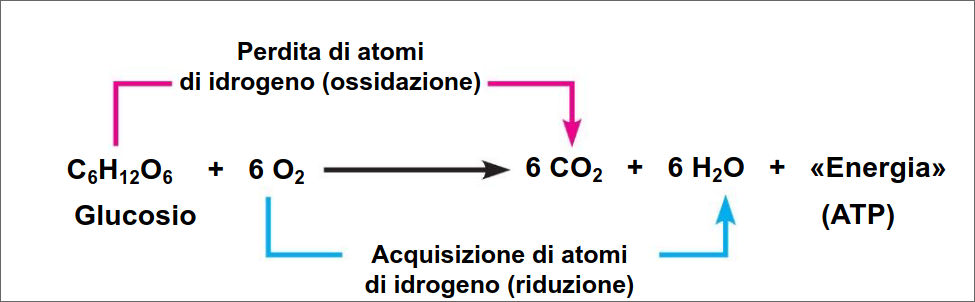
\includegraphics[width=0.85\textwidth]{./resources/resp.png}
    \end{figure}
    \end{center}
\end{snippet}

\begin{snippet}{respirazione-cellulare-expl}
    La respirazione cellulare serve a spaccare i legami di una molecola grande
    (tanti legami) e trasferirne l'energia chimica nell'ATP.
    Gli atomi, H\({}_2\)O e CO\({}_2\) sono scarti. Gli elettroni servono nel processo per caricare l'ATP, per poi
    essere scartati.
\end{snippet}

\begin{snippetdefinition}{mitocondrio-definizione}{Mitocondrio}
    Il \textit{mitocondrio} è un organello nella cellula dove avviene parte della respirazione cellulare.
\end{snippetdefinition}

\plain{Il mitocondrio è composto da due membrane, dividendosi in una parte interna ed esterna.}

\begin{snippetdefinition}{creatina-definizione}{Creatina}
    La \textit{creatina} è una molecola che possiede un fosfato, il suo scopo è quello di aumentare la produzione di ADP.
\end{snippetdefinition}

\begin{snippet}{respirazione-step}
    le 3 tappe della respirazione cellulare sono
    \begin{enumerate}
        \item \textbf{Glicolisi}
        \item \textbf{Cliclo di Krebs} (all'interno del mitocondrio)
        \item \textbf{Fosforilazione ossidativa} (gradienti fra lo spazio intermembranan e lo spazio interno del mitocondrio)
    \end{enumerate}
\end{snippet}

\begin{snippetdefinition}{glicolisi-definizione}{Glicolisi}
    La \textit{glicolisi} è una serie di reazioni chimiche che spaccano il glucosio in 2 \textit{piruvati} (\(C_3H_6O_3\)).
\end{snippetdefinition}

\begin{snippet}{f864100d-b046-461a-a7d7-21d6c0e22c54}
    Questo procedimento produce (poco) ATP dallo spaccamento e libera elettroni.
    Gli elettroni liberati vengono presi dall'NAHD (molecole di trasporto degli elettroni
    che diventa FADH\({}_2\))
    che le trasportano nella cellula.

    Il piruvato entra nel ciclo di Krebs, dove esce il CO\({}_2\) per produrre l'Acetil-coenzima A.
    L'Acetil-coenzima A viene spaccato, producendo una piccola quantità di ATP.
    Vengono quindi spaccati tutti gli atomi, tenendo solo gli elettroni che vanno nel terzo processo.

    Gli elettroni prodotti si avviano verso il mitocondrio. La cellula è interessata a portare
    gli \(H^+\) contro grandiente verso lo spazio fra le 2 membrane.
    Per trasportarli contro gradiente viene sfruttata l'energia degli elettroni che si muovono in saltando fra le proteine.

    Gli elettroni vengono successivamente presi dall'ossigeno, che li usa per legare con gli \(H^+\) e formare
    acqua.
\end{snippet}

\section{Fermantazione alcolica}

\begin{snippet}{d21b6e74-c162-4339-8caa-62103156b1fa}
    La fermantazione alcolica avviene in assenza di ossigeno e viene svolta prevalentmeente dagli lieviti (fungi unicellulari).
    Lo lievito fa la fermentazione per vivere e svolgere le sue funzioni metaboliche.
    
    Dopo aver prodotto l'energia, è necessario sbarazzarsi del piruvato protonato (acido piruvio),
    viene quindi spaccato e scaricato nell'aria come Etanolo e CO\({}_2\).
    % CO2 e Etanolo con REDOX scaricano NADH
\end{snippet}

\section{Fermantazione lattica}

\begin{snippet}{966e3037-9b93-4ccb-8797-7939a6ca6059}
    La fermentazione lattica viene svolta da alcuni organismi come batteri.
    Gli umani la svolgono dopo uno sforzo muscolare.
    Il piruvato viene convertito in acido lattico (scarto), che viene poi smaltito dal fegato con ATP.
\end{snippet}

\end{document}